Off-line trained surrogate models are built prior to the 
evolution and are trained primarily on a dataset of training 
patterns, which cover the entirety of the design space and are 
collected via the implementation of various DoE techniques. The 
training process is disconnected from the evolution and, thus, this 
method is described as static. MAEAs with off-line training can be 
decomposed in the following steps:

\begin{OFFL}
\item \textbf{Design of Experiments (DoE)} \\
One of the various DoE techniques is applied and the sampling 
process initiates, which involves the selection of $n_{doe}$ 
observations $\vec{χ} \! \in \! \mathbb{R}^{n_{β}}$ from within 
the imposed bounds of the design space. Subsequently, the necessary 
objective function values $\vec{f}(\vec{χ})$ are computed on the 
PSM. Consequently, the resulting $n_{doe}$ $(\vec{χ},\vec{f}
(\vec{χ}))$ observed pairs are archived in a database reserved for 
the training of the metamodels which is referred to as metamodel 
database (MDB). Any untried point in the design space that is not 
archived in the MDB, i.e. each candidate solution, is denoted by 
$\vec{β} \in \mathbb{R}^{n_{β}}$.

\item \textbf{Training of the metamodel}\\
The $n_{t}$ archived $(\vec{χ},\vec{f}(\vec{χ}))$ pairs  are used 
in the training of the metamodel. In the first optimization cycle, 
the number of training patterns $n_{t}$ is equal to the $n_{doe}$ 
observations. DoE techniques are applied mainly in MAEAs with 
off-line training and are used to collect training patterns from 
the entirety of the design space, resulting in the construction of 
a global metamodel. 

\item \textbf{Implementation of EAs}\\
The optimization process initiates subsequently via the
use of the EASY software that implements EAs. The evolution 
follows the process described in section \ref{section:EAs} 
with one main variation; the offspring evaluation in step 2 
(EAs-2) is performed via the use of the trained surrogate 
model. The metamodel serves as a black box that approximates $λ$ 
individuals, where $λ$ is the number of offspring in the 
$P_{λ}^{g}$ set, and provides the corresponding prediction of 
the objective function value \scalebox{0.86}{%
$\hat{\vec{f}}(\vec{β})$}, $\forall \vec{β} \!\in \!P_{λ}^g$. Each 
prediction \scalebox{0.86}{%
$\hat{\vec{f}}(\vec{β})$ } is assigned a scalar fitness function 
value $\hat{Φ}(\vec{β})$, which in MOO problems is based on 
dominance criteria and $\hat{Φ}(\vec{β}) \!\equiv \!\hat{f}
(\vec{β})$ in SOO. The criterion that prohibits EAs from exceeding 
a selected number of evaluations is accordingly modified to fit the 
trivial computational cost of the metamodel.  

\newpage
%----------------------------------------------------------------

%\begin{figure}[h]
%\centering
%\begin{tikzpicture}[scale=0.6, every 
%node/.style={font=\sffamily}, align=center]
%\draw[thick,->, color=blue!70] (-7,2) -- (-5,2) 
%node[anchor=south east, xshift = -0.4 cm, color = black!100] 
%{$\vec{β}$}; 
%\filldraw [color=gray!40] (0,0) rectangle (-4,4);
%\draw (-2,3) node[rotate=0, anchor=north]{SMT \\ source code};
%\draw[thick,->, color=blue!70] (1,2) -- (3,2) 
%node[anchor=south east, xshift = -0.2 cm, color = black!100] 
%{$\hat{f}(\vec{β})$};
%\draw [red,thick,dashed] (-10,-0.75) rectangle (6.5,5) 
%node[anchor=north east]{step EAs-3};
%\end{tikzpicture}
%\caption{Use of metamodel as a black box}
%\end{figure}

\item \textbf{Re-evaluation on the PSM}\\
The re-evaluation process initiates once the evolution 
has been completed and the optimal candidate solutions have 
been found. The best candidate solution in SOO or a set of 
$λ_{α}^{(i)}$ non-dominated solutions in MOO, residing in the 
$P_{e}^{(i)}$ temporary set, are re-evaluated using the exact PSM. 
Index \textit{i} is used to denote the current cycle of the MAEA 
algorithm using off-line training. 

\item \textbf{Termination}\\
The deviation between the metamodel and the PSM evaluated 
objective function values determines the convergence of the 
MAEA-based optimization. In case the convergence criteria are not 
met, the optimal candidate solution/s residing in 
the $P_{e}^{(i)}$ set at the end of the evolution or some others 
arbitrarily selected individuals are used to update the 
existing MDB. The outcome of their evaluation, i.e. 
$\vec{f}(\vec{β})$, $\forall \vec{β} \!\in \!P_{e}^{(i)}$, is 
subsequently added to the updated MDB and the $i_{th}$ evolution 
terminates. The next cycle of the optimization initiates 
starting from step 1 (OFFL-1) and index \textit{i} is set to 
$i \leftarrow i+1$. The evolution's inability to yield an 
optimal solution is indicative of a poorly trained surrogate 
model and, therefore, an improved metamodel needs to be 
trained. Consequently in step 1 (OFFL-1) of the $(i+1)_{th}$ 
cycle, DoE techniques are implemented to select $n_{new\_doe}$ 
new points and in the following step (OFFL-2) a new metamodel 
is built on $n_{t}$ training patterns, where:
\begin{equation}\label{off_line_nt}
n_{t} = n_{doe} + \sum_{i=0}^{i} \left( λ_{α}^{(i)} +
n_{new\_doe} \right) 
\end{equation}
\\[-0.1cm]
where $λ_{α}^{(i)}$ is the number of elites selected in the 
$i_{th}$ generation and $n_{new\_doe}$ a user-defined number of 
sample points that is sampled via DoE techniques at the start 
of each optimization cycle in order to fill the MDB and improve 
the fitting of the metamodel. The updated number of sample points 
will be denoted by $n_{doe}^{'}$ for simplicity, where:
\begin{equation}
n_{doe}^{'} = n_{doe} + \sum_{i=0}^{i} \left(n_{new\_doe} \right)
\end{equation} 

The aforementioned steps outline the function of MAEAs with 
off-line trained metamodels and will be subsequently combined into 
the flowchart form of figure \ref{fig:offline_flowchart}.
\end{OFFL} 

\newpage
%--------------------------------------------------------


\begin{figure}[h!]
\centering
\begin{adjustbox}{width=0.9\textwidth,height= 
1\textheight,keepaspectratio}
\begin{tikzpicture}[node distance=1.7cm,
    every node/.style={fill=white, font=\sffamily}, 
    align=center]
\node (start) [startstop] {Start};
\node (pro0) [process, below of=start, yshift=0.2cm] 
{$i = 0$};

\node (pro1) [process, below of=pro0, yshift=0.2cm] 
{$DoE \rightarrow \mathbf{X}$};

\node (pro2) [process, below of=pro1, yshift=-0.4cm] 
{$g=0$ \\ Evaluation on the PSM $\rightarrow$
\\ $ n_{t}$ $(\vec{χ}, \vec{f}(\vec{χ}))$ pairs in MDB \\
$\rightarrow$ train metamodel};

%------------------EA loop--------------------------------
\node (init1) [process, below of=pro2, yshift=-0.5cm] 
{Initialize $P_{λ}^{g}$};

\node (pro3) [process, below of=init1, yshift=0.2cm] 
{Compute $\hat{\vec{f}}(\vec{β})$};

\node (dec3) [decision, below of=pro3, yshift=-0.5cm] 
{$j < λ$};

\node (pro4) [process, below of=dec3, yshift =-0.5cm] 
{Computation of $\hat{Φ}(\vec{β})$};

\node (pro5) [process, below of=pro4] 
{Update elites $\rightarrow \!P_{α}^{g+1}$};

\node (pro6) [process, below of=pro5, yshift=-0.1cm]
{Parent \\ selection $\rightarrow \!P_{μ}^{g+1}$};

\node (pro7) [process, below of=pro6, yshift=-0.1cm] 
{Crossover and \\ mutation $\rightarrow \!P_{λ}^{g+1}$};

\node (dec1) [decision, below of=pro7, yshift=-1.2cm] 
{EA \\ Termination};
%-------------------------------------------------------------

\node (pro8) [process, right of=dec1, xshift=4cm] {Evaluation of \\ 
$P_{e}$ on the PSM};

\node (dec2) [decision, right of=init1, xshift=4cm] 
{Convergence};

\node (pro9) [process, above of=dec2, yshift = 2.6cm] 
{Update MDB \\ with $P_{e}$};

\node (stop) [startstop, right of=dec2, xshift=1.5cm]
{Stop};

\draw [arrow] (start) -- (pro0);
\draw [arrow] (pro0) -- (pro1);
\draw [arrow] (pro1) -- (pro2);
\draw [arrow] (pro2) -- (init1);
\draw [arrow] (init1) -- (pro3);
\draw [arrow] (pro3) -- (dec3);
\draw [arrow] (dec3) -- (pro4);
\draw [arrow] (pro4) -- (pro5);
\draw [arrow] (pro5) -- (pro6);
\draw [arrow] (pro6) -- (pro7);
\draw [arrow] (pro7) -- (dec1);
\draw [arrow] (pro8) -- (dec2);

%-----------arrow dec1------------------
\draw [arrow] (dec1.east) -- node[anchor=south, 
xshift = -0.5cm] {yes}(pro8.west);
\draw [->][arrow] (dec1.west) -- ++(-2,0) -- ++(0,12.6) 
-- ++(2,0) -- node[xshift=-2cm,yshift=-3.5cm, text 
width=2.5cm]{$g = g +1 $}(pro3.west);

%-----------arrow dec2-------------------
\draw [arrow] (dec2.north) -- node[anchor=west]{no} 
(pro9);
\draw [arrow] (dec2) -- node[anchor=south]{yes}(stop);
\draw (-2.5,-20.8) node[anchor=north]{no};

%------------draw rectangle--------------
\draw [red, thick, dashed] (-4.7,-23.3) rectangle 
+(8.2,16.9);
\draw [red] (-3.8,-22.6) node[anchor=north]{EA loop};

%------------draw pro9-------------------
\draw [arrow] (pro9) -- node[anchor=south]{$i=i+1$}(pro1);

%-----------arrow dec3-------------------
\draw [arrow] (dec3.east) -- ++(1.5,0) -- ++(0,2.2) 
-- ++(-1,0) -- node[anchor=north, xshift = 1cm, 
yshift=-0.9cm] {$j=j+1$}(pro3.east);
\draw (0.4,-12) node[anchor=north]{no};
\draw (1.5,-11.2) node[anchor=north]{yes};


\end{tikzpicture}
\end{adjustbox}
\caption{Flowchart of MAEAs using off-line trained 
metamodels}
\label{fig:offline_flowchart}
\end{figure}

\newpage
%--------------------------------------------------------


\section{Design of Experiments (DoE)}
The predominant characteristic of off-line trained MAEAs is the 
construction of a single global surrogate model 
\cite{global_metamodel}. The majority of necessary patterns 
for the training of this global metamodel are collected via the 
use of various Design of Experiments (DoE) techniques that sample 
the entirety of the design space. DoE is a statistical tool used 
for analyzing the interactions between the parameters that 
effect the performance of a system and controlling them 
in order to optimize its performance\cite{DOE,DOE1,DOE2}.
%In metamodel construction, DoE techniques are implemented 
%to map the response $\vec{f}(\vec{χ}) \!\in \!\mathbb{R}^{n}$ to 
%each observation $\vec{χ}$. 
The most commonly used DoE techniques and the ones studied in this 
thesis are the following: 

\begin{enumerate}
\item \textbf{Random sampling} \\
The most common technique of removing bias from a design is 
randomization, which gives each sample point $\vec{χ} \!= \! 
[χ_{1}, χ_{2}, \hdots, χ_{n_{β}}] \in \mathbb{R}^{n_{β}}$ 
equal probability of being selected from the design 
space \cite{Random}, as shown in figure \ref{fig:random}. 

\vspace{-4mm}
  
\begin{figure}[h!]
    \centering
    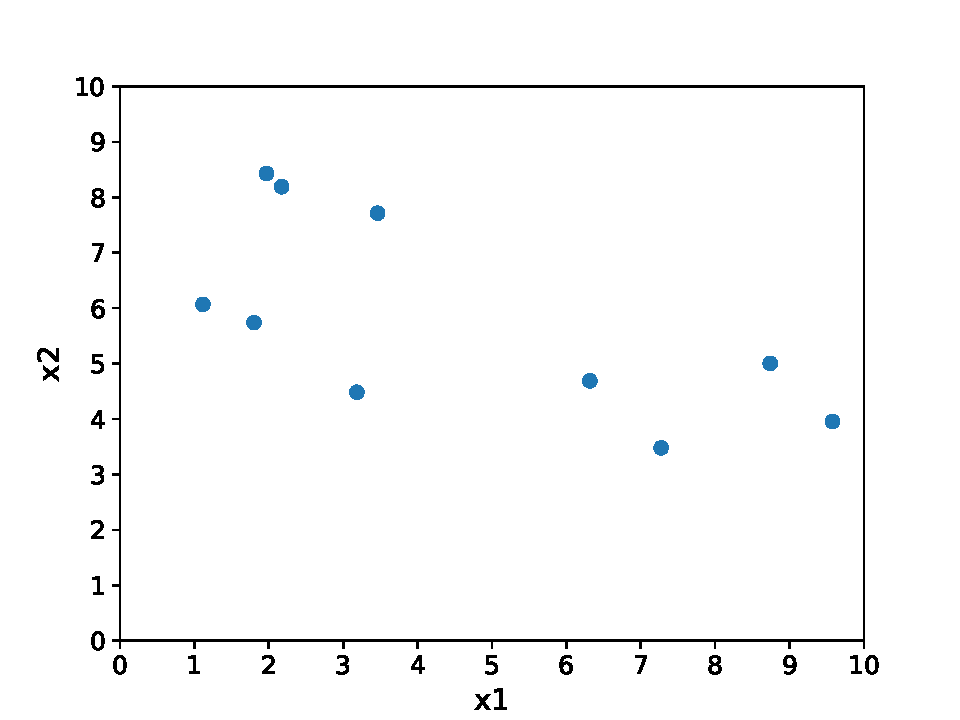
\includegraphics[width=0.47\textwidth]{random_SMT.pdf} 
    \caption{Random design in 2D space for $n_{doe} \!= \!10$ 
    sample points}
    \label{fig:random}   
\end{figure}

\item \textbf{Latin Hypercube Sampling (LHS)}  \\ 
A square grid containing a single sample point $\vec{χ} \in 
\mathbb{R}^{2}$ per row and column is called a Latin Square.
The generalization of this design in $n_{β} \!> \!2$ dimensions 
results in the creation of a Latin Hypercube (LH)\cite{Latin 
Hypercube}. A Latin Hypercube Design (LHD) aims to improve the 
coverage of the design space and eliminate the probability of two 
coinciding sample points and is created via the implementation of 
LHS\cite{LHS, LHS method} scheme. In LHDs, the design space in 
each dimension is stratified into $n_{doe}$\footnote{The original 
design ($i=0$) consists of $n_{t} = n_{doe}$ points, while a 
separate design is constructed for every $n_{new\_doe}$ points 
sampled. Without loss of generality, we assume from this point 
forward that in the description of DoE we refer to the original 
design of $n_{doe}$ points.} equiprobable and non-overlapping 
intervals\cite{LHS}, called strata. Subsequently, $n_{doe}$ 
distinct values are selected, one from each stratum, and are 
paired to form the components $χ_{1}, χ_{2}, \hdots, χ_{n_{β}}$ of 
each sample vector $\vec{χ} \!\in \!\mathbb{R}^{n_{β}}$. As a 
result of the stratification, the LHD consists of $n_{doe}$ 
distinct sample points and can be written as a $n_{doe} \times 
n_{β}$ matrix $\mathbf{X} = [\vec{χ}_{1}, \vec{χ}_{2}, \hdots, 
\vec{χ}_{n_{doe}}]^T$, where each component $\vec{χ}_{i} = [χ_{i,
1}, χ_{i,2},\hdots, χ_{i,n_{β}}]$ represents an observation 
$\vec{χ} \in \mathbb{R}^{n_{β}}$. LHDs can be enhanced with 
several optimality construction criteria, some of which are 
presented here \cite{preprint_SMT,pyDOE}:

\newpage
%-----------------------------------------------------------


\begin{enumerate}
\item \textbf{Centered LHD} \\
This construction criterion centers the selected values from within 
each hypercube, as shown in figure \ref{fig:centered_LHD}. 

\vspace{-2mm}

\begin{figure}[h!]
    \centering
    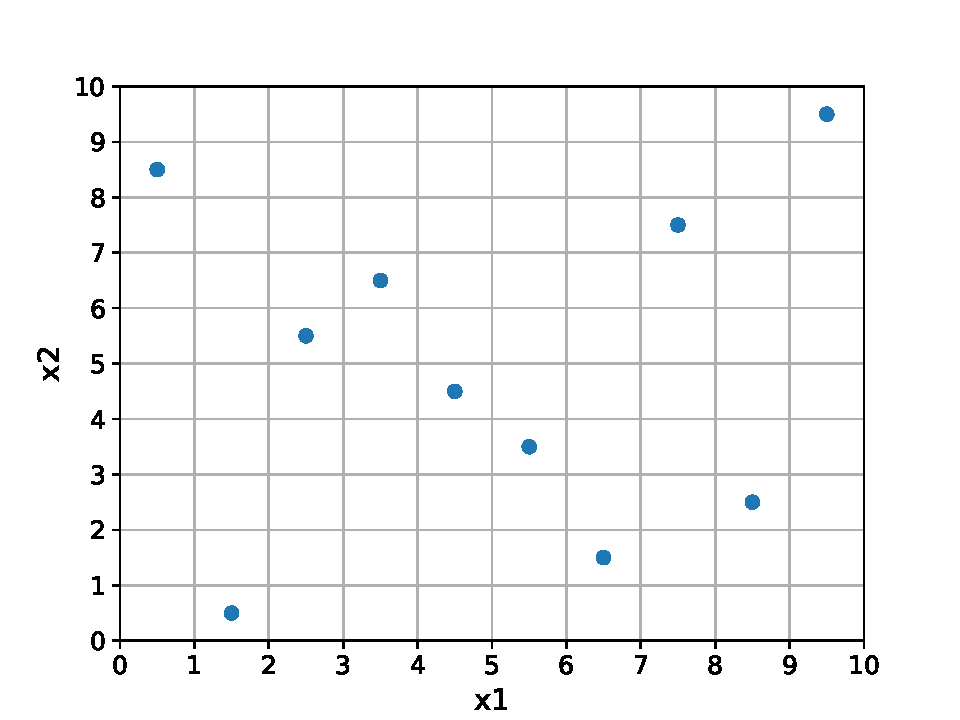
\includegraphics[width=0.5\textwidth]{criterion_c.pdf}    
    \caption{Centered LHD in 2D space. The grid has been modified 
    to facilitate the visualization of $n_{doe} = 10$ strata in 
    each dimension.}
    \label{fig:centered_LHD}
\end{figure}
    
\item \textbf{Maximin LHD} \\
This construction criterion was introduced by Johnson et al.
\cite{maximin} based on the idea that the Euclidean distance 
between sample points should be used as a metric for design 
construction. A maximin design, denoted by $S_{Mm}$, 
guarantees that every pair of points will never coincide by 
maximizing the minimum distance between them \cite{maximin2}.
\begin{equation}\label{maximin}
\max\limits_{S \subset \mathbb{R}^{n_{β}}} 
\min\limits_{\vec{χ}_{i}, \vec{χ}_{j} \in S} d(\vec{χ}_{i}, 
\vec{χ}_{j} ) = 
\min\limits_{\vec{χ}_{i}, \vec{χ}_{j} \in S_{Mm}} 
d(\vec{χ}_{i}, \vec{χ}_{j}) 
\hspace{3mm} ,\forall i,j \in [1,n_{doe}]
\end{equation}

Each selected point $\vec{χ} \!\in \!S$, where $S$ the selected 
design set, is the center of a sphere, the radius of which is 
calculated by the algorithm that produces the maximin design 
described by eq. \ref{maximin}. Consequently, the final design 
contains $n_{doe}$ non-overlapping spheres. In a maximin LHD, the 
sample points must furthermore be selected from within within each 
hypercube, as shown in figure \ref{fig:maximin_LHD}.

\vspace{-2mm}

\begin{figure}[h!]
    \centering
    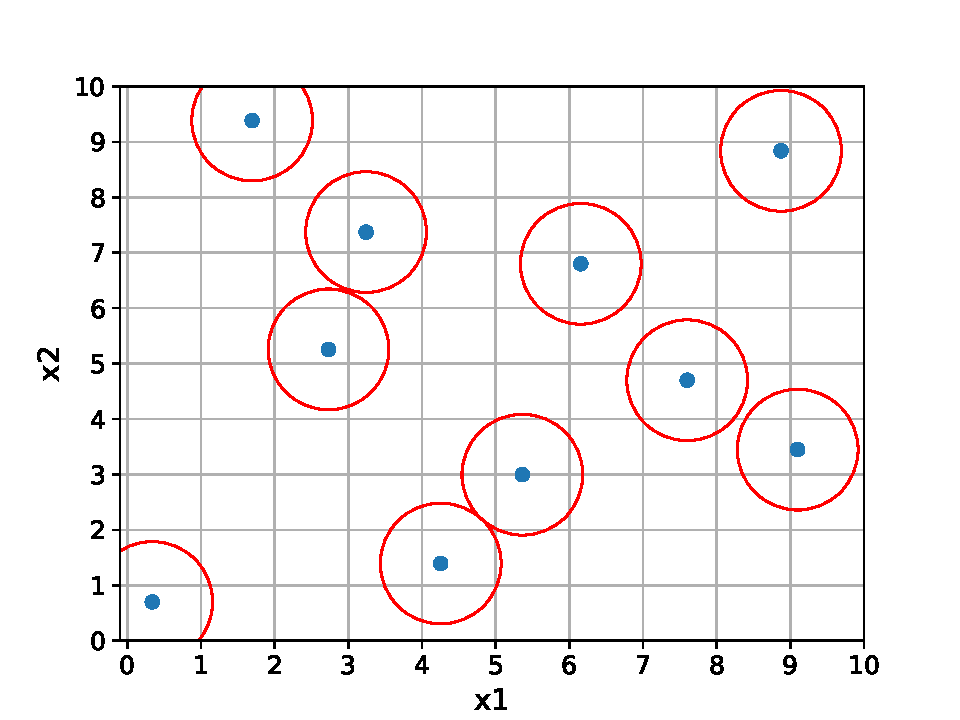
\includegraphics[width=0.5\textwidth]{criterion_m.pdf}    
    \caption{Maximin LHD in 2D space for $n_{doe} = 10$ 
    sample points}
    \label{fig:maximin_LHD}
\end{figure}

\newpage
%--------------------------------------------------------------


\item \textbf{Maximin Centered LHD} \\
Similar to maximin LHD with the exception that the selected sample 
points are centered within each hypercube, as shown in figure 
\ref{fig:maximin_centered_LHD}.

\vspace{-4mm}

\begin{figure}[h!]
    \centering
    \includegraphics[width=0.47\textwidth]{criterion_cm.pdf}    
    \caption{Maximin centered LHD in 2D space for $n_{doe} = 10$ 
    sample points}
    \label{fig:maximin_centered_LHD}
\end{figure}

\item \textbf{Maxent LHD} \\
Information entropy as proposed by Shannon \cite{entropy} is 
directly associated to the level of information available from a 
design. Shewry and Wynn \cite{max_entropy} showed that maximizing 
the entropy of the response distribution at the sampled design 
sites $\mathbf{X}$ is equivalent to maximizing the gain of 
information of the response distribution at any untried location of 
the design space. If the response distribution is given by a 
stationary Gaussian process $Y(\cdot)$ with mean $μ_{Y}$, 
variance $σ^{2}$ and correlation function $R(\cdot)$, then the 
optimal design $S \!\subset \!\mathbb{R}^{n_{β}}$ can be found by 
maximizing the simplified entropy of the distribution of the 
responses at the design sites, as such:  
\begin{equation}
\max\limits_{\vec{χ}_{i}, \vec{χ}_{j} \in S} - 
ln\left[det\mathbf{R}(\vec{χ}_{i}, \vec{χ}_{j})\right]
\end{equation}
\\[-2mm]
where $\mathbf{R}(\vec{χ}_{i}, \vec{χ}_{j}) = \prod_{l=1}^{n_{χ}}
exp( -\theta_{l} \left| χ_{i,l} - χ_{j,l} \right|^{q})$ and $q$ a 
positive integer with values 1 or 2, corresponding to an 
exponential or a Gaussian kernel, respectively. The parameters 
$θ_{l}$ denote the degree of correlation between training points 
w.r.t. each design dimension $l \!\in \![1,n_{β}]$. In a maxent 
LHD, the sample points must furthermore be selected from within 
within each hypercube, as shown in figure \ref{fig:maxent_LHD}.

\vspace{-4mm}

\begin{figure}[h!]
    \centering
    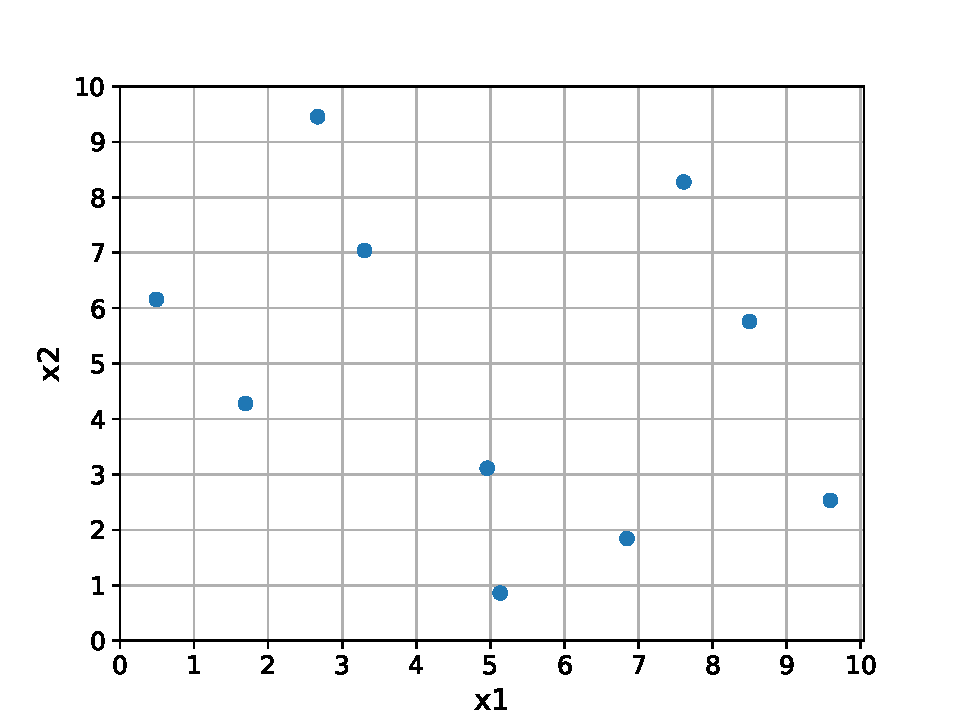
\includegraphics[width=0.47\textwidth]{criterion_corr.pdf}    
    \caption{Entropy LHD in 2D space for $n_{doe} = 10$ 
    sample points}
    \label{fig:maxent_LHD}
\end{figure}

\newpage
%--------------------------------------------------------------


\item \textbf{Enhanced Stochastic Evolutionary (ESE) LHD} \\
This criterion is an enhancement to the existing global 
search, stochastic evolutionary (SE) algorithm, originally 
developed by Saab and Rao\cite{SE}. The need to further 
reduce the computational cost of SE resulted in the creation 
of Enhanced Stochastic Evolutionary algorithm (ESE
)\cite{ESE}. This new approach is based on utilizing 
efficient methods for evaluating various space-filling criteria, 
namely $φ_{p}$, entropy and centered $L_{2}$ discrepancy 
criterion. The first criterion was proposed by Morris and Mitchel 
(1995)\cite{fp criterion} and is an extension of the maximin 
criterion. $L_{2}$ discrepancy is the most common expression of 
$L_{p}$ discrepancy, which is a metric of non-uniformity of a DoE. 
The formula used to describe centered $L_{2}$ or $CL_{2}$ 
discrepancy was proposed by Hickernell (1998)\cite{discrepancy}. 
The minimization of $CL_{2}$ discrepancy results in a uniform 
design. ESE combines these three aforementioned space-filling
criteria to construct an optimal design. In a ESE LHD, the sample 
points must furthermore be selected from within within each 
hypercube, as shown in figure \ref{fig:ESE_LHD}.

\begin{figure}[h!]
    \centering
    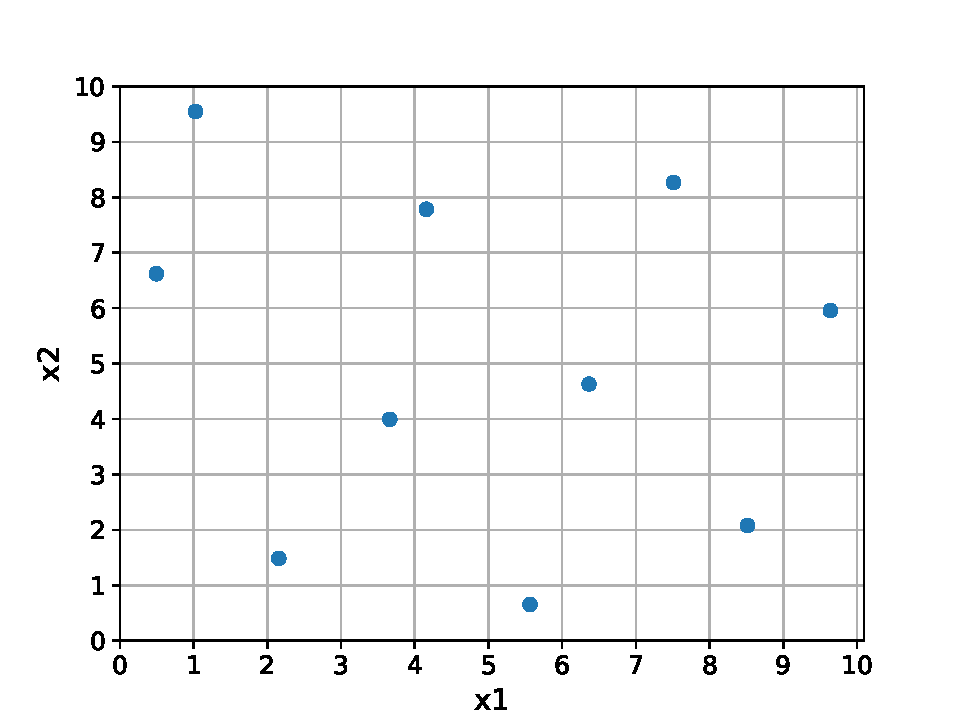
\includegraphics[width=0.5\textwidth]{criterion_ese.pdf}    
    \caption{ESE LHD in 2D space for $n_{doe} = 10$ 
    sample points}
    \label{fig:ESE_LHD}
\end{figure}

\end{enumerate}

The quality of the LHD affects the convergence of the 
MAEA-based optimization process and therefore selecting the 
most cost-efficient construction criterion of an LHD is essential 
for the success of this method. An analysis performed in appendix 
\ref{appendix:constr_crit}, concluded that ESE LHDs are the most 
suitable for the purpose of this thesis and therefore the LHS 
scheme is modified accordingly to produce such designs.

\newpage
%--------------------------------------------------------


\item  \textbf{Factorial sampling}\\
In a factorial design, the relative importance of each design 
variable (factor) on the objective function is tested by 
replicating all the possible combinations of the factors. 
Each possible combination is replicated in a run of the 
design with a total of $n_{doe}$ runs being performed. Each 
factor is assigned a number of discrete values in the [-1,1] 
range, called levels, where high and low influence are 
assigned a level of 1 and -1 respectively\cite{Factorial}. 
The change in response caused by an alteration in the level 
of each factor can, therefore, be correlated with the 
relative importance of each factor. The complete replicate 
of a factorial design that contains all possible combinations 
between $n_{β}$ factors is called a Full Factorial Design 
(FFD). A conventional FFD is performed at 2 levels, i.e 1 
and -1, which results in $n_{doe} = 2^{n_{β}}$ possible 
combinations\cite{Full_Factorial2}. However, the number of 
factorial runs $n_{doe}$ is user-defined, i.e. 
$n_{doe} \! \neq \! 2^{n_{β}}$ or $n_{doe} \neq 3^{n_{β}}$, 
and the cost of constructing a FFD grows exponentially 
as the number of factors increases. In order to overcome the 
imposed restrictions, interactions between factors that yield
the lowest response are neglected. The resulting design is a  
fractional factorial design\cite{Fractional Factorial}; such a 
design is depicted in the following case for $n_{doe} = 10$
sample points in figure \ref{fig:Full_Fact_example}:

\begin{table}[h!]
\centering
\begin{tabular}{|c|c|c|c|c|c|}
\toprule
\rowcolor{gray!20} \textbf{Levels}
 & \textbf{-1} & \textbf{-0.5} & \textbf{0} 
 & \textbf{0.5} & \textbf{1} \\ 
\midrule
\textbf{$χ_{1}$} & 6 & 7.33 & - & 8.66 & 10 \\ 
\hline 
\textbf{$χ_{2}$} & 150 & - & 175 & - & 200 \\ 
\bottomrule
\end{tabular}
\end{table} 

\begin{figure}[h!]
    \centering 
    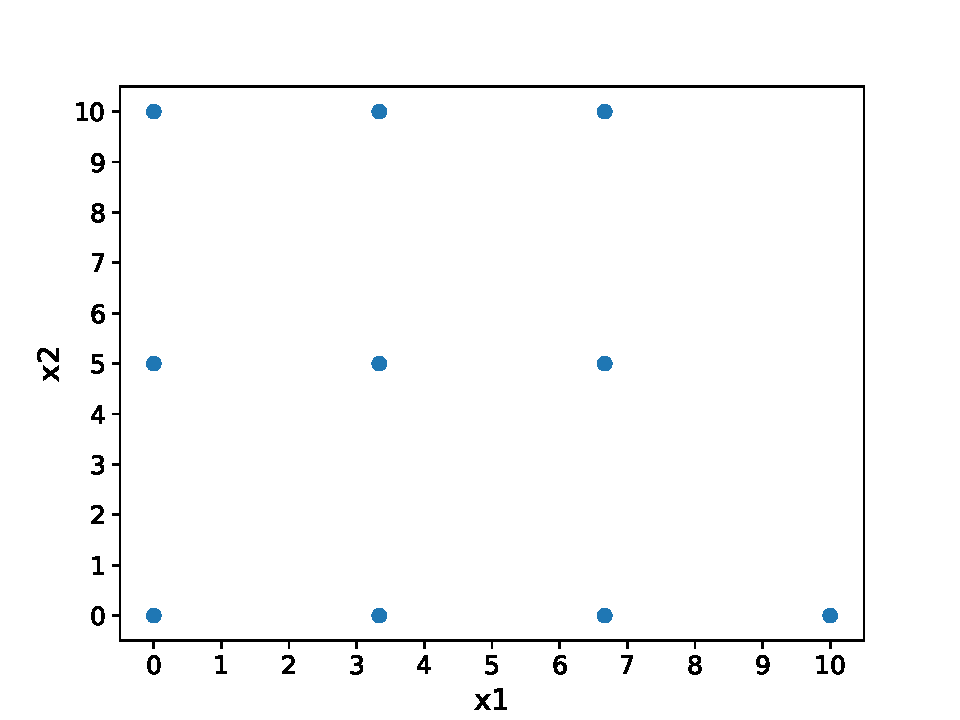
\includegraphics[width=0.5\textwidth]
    {full_factorial_SMT.pdf} 
    \caption{Example of Factorial design for 2 design 
    variables with $n_{doe} = 10$ sample points}
    \label{fig:Full_Fact_example}
\end{figure} 

\end{enumerate}

\newpage
%-------------------------------------------------------


\subsection{Comparison between DoE construction schemes}
The selection of a suitable design is an essential step to
the training of a surrogate model. For that reason the 
available DoE construction schemes are evaluated w.r.t. their
effect on the training process of the metamodel. The 
comparison is limited to Factorial and LH designs, since they 
tend to be the most reliable in overall coverage of the design 
space and especially in the selection of a representative sample 
from the total population set. Random designs are eliminated from 
the assessment process, since they are considered unfit for large 
population sets due to equiprobable selection of each individual. 
Optimality space-filling criteria are not utilized in random 
designs and the outcome is a design that either contains a number 
of similar sample points or omits significant sample points 
that are of great importance to the training of the 
surrogate model \cite{Random}.

The first difference between the two remaining DoE 
construction schemes is detected in the selection process of 
sample points. In both full and fractional factorial designs, the 
sample points are distributed as evenly as possible in the 
$n_{β}$-dimensional design space, utilizing its full 
capacity. In LHDs, the design space is stratified and the 
sample points are selected from within the created intervals 
via the use of some space-filling construction criterion. 
For up to $n_{β} = 3$ design variables the resulting designs can 
be replicated in 3D space as depicted in figure 
\ref{fig:LH_vs_FD_in3D}; in this example the design space is 
created by the bounds of each design variable in eq. 
\ref{pseudo_aircraft}.

 \begin{figure}[h!]
    \centering
    \begin{subfigure}[b]{0.50\textwidth}
    \centering
    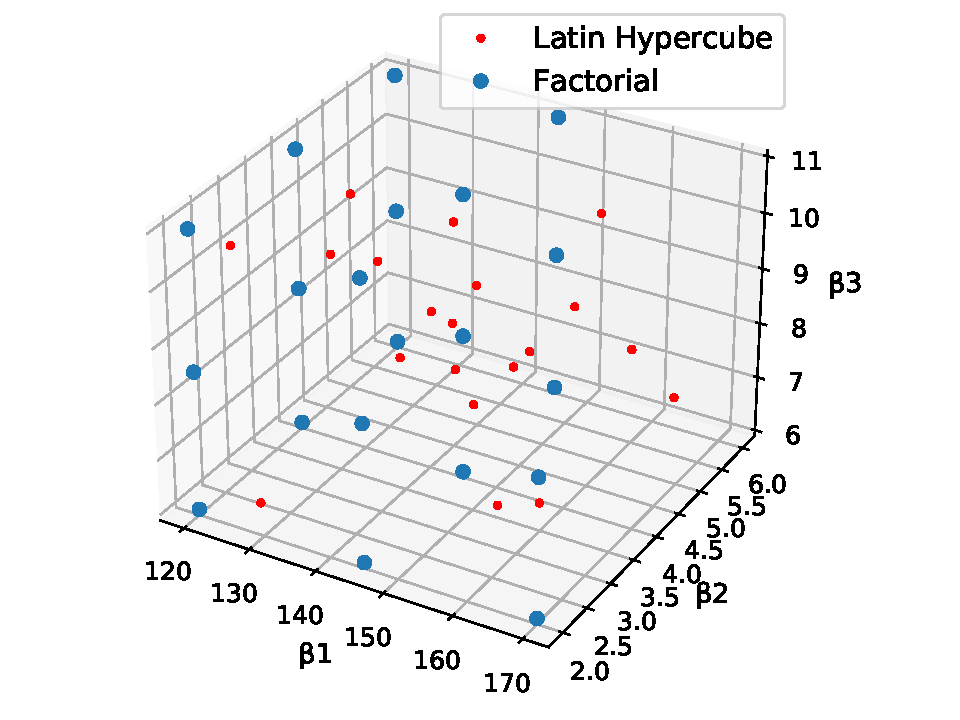
\includegraphics[width=\textwidth]{lhs_vs_fullf1.pdf}
    \caption{3D design space} 
    \end{subfigure}  
\hfill
\begin{subfigure}[b]{0.49\textwidth}
    \centering
    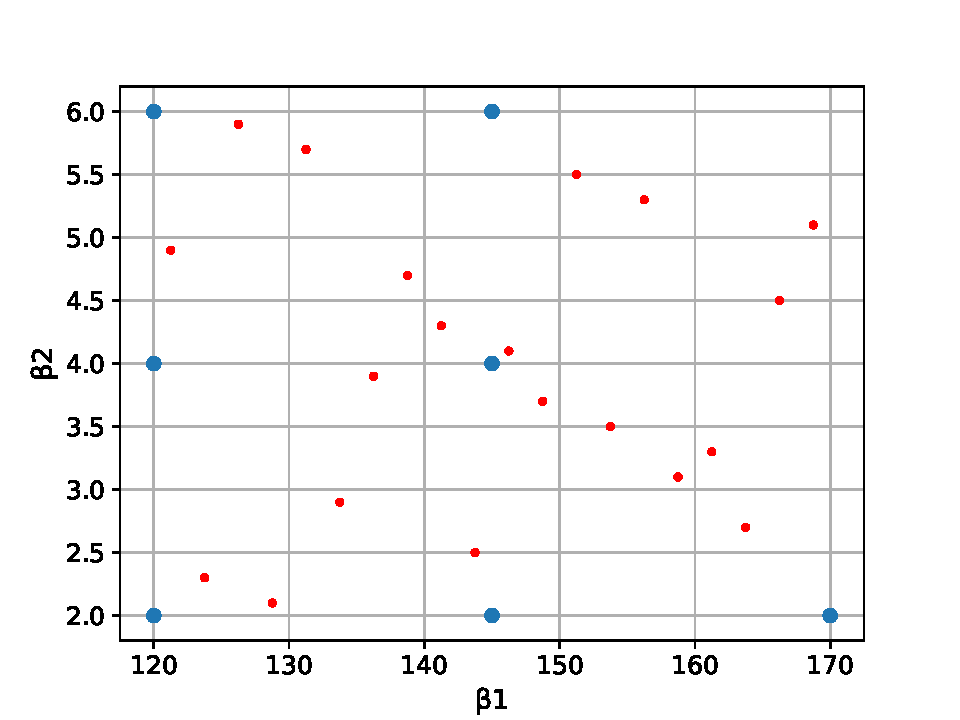
\includegraphics[width=\textwidth]{lhs_vs_fullf2.pdf} 
    \caption{2D contour surface along $χ_{1}$, $χ_{2}$ plane}
    \end{subfigure}
\hfill
\begin{subfigure}[b]{0.49\textwidth}
    \centering
    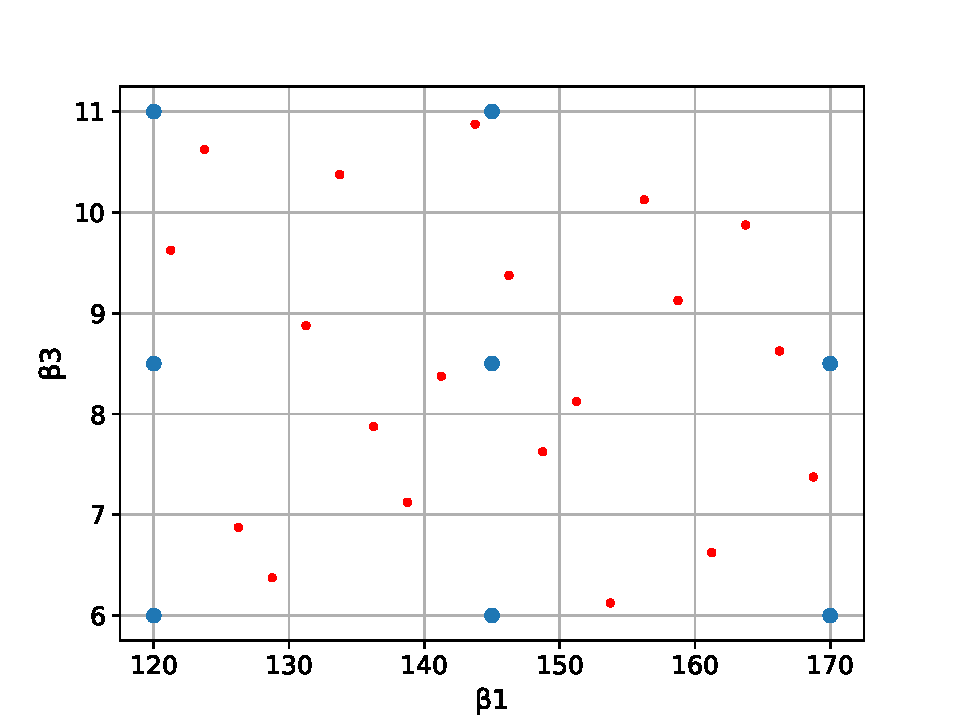
\includegraphics[width=\textwidth]{lhs_vs_fullf3.pdf} 
    \caption{2D contour surface along $χ_{1}$, $χ_{3}$ plane}
    \end{subfigure}
\hfill
\begin{subfigure}[b]{0.49\textwidth}
    \centering
    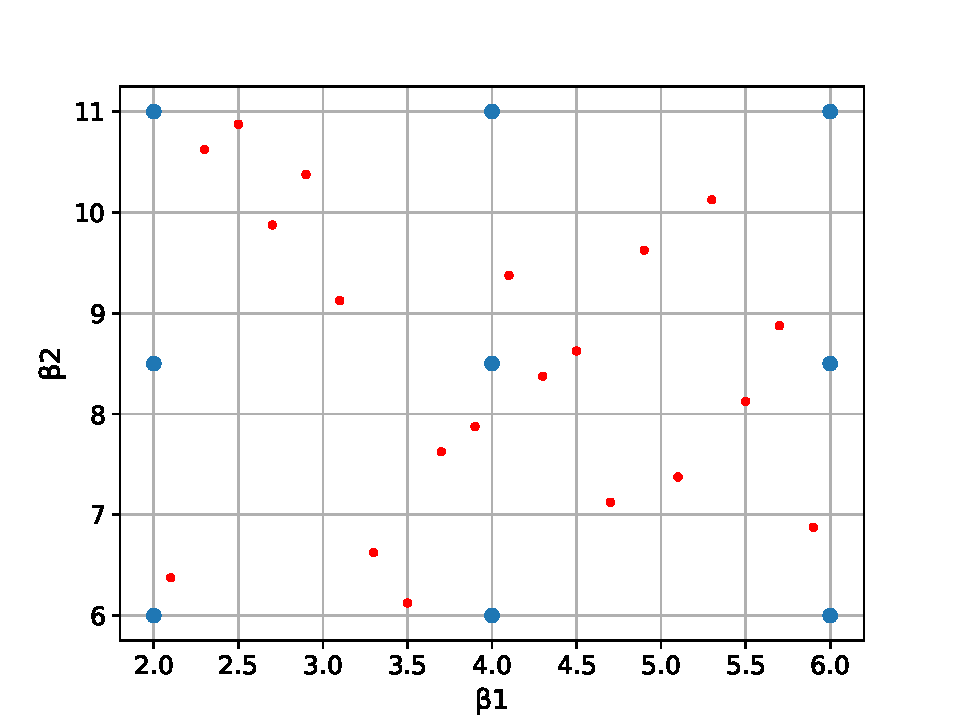
\includegraphics[width=\textwidth]{lhs_vs_fullf4.pdf}
    \caption{2D contour surface along $χ_{2}$, $χ_{3}$ plane} 
    \end{subfigure}
\caption{Factorial and LH designs in 3D design 
space} 
\label{fig:LH_vs_FD_in3D}      
\end{figure}

\newpage
%-----------------------------------------------------------


The implementation of factorial sampling in 3D space for 
$n_{doe} = 20$ runs results in the creation of a fractional 
factorial design, which disregards a large section of the design 
space. For the same number of runs, on the other hand, LHS scheme 
spreads sample points optimally across the design space and yields, 
for this reason, better designs. In LHDs furthermore, the MDB is 
more diverse and complete, since it consists of $n_{doe}$ distinct 
values, unlike in factorial designs where the influence of each 
design variable is tested on $κ_{l} < n_{doe}$ levels each. The 
responses of $n_{doe}$ sample points can be written as a $n_{doe} 
\times n$ matrix $\mathbf{F} = [\vec{f}_{1}, \vec{f}_{2}, \hdots, 
\vec{f}_{n_{doe}}]^{Τ}$, where each component $\vec{f}_{i} = 
[f_{i,1}, f_{i,2}, \hdots, f_{i,n}]$ represents a response $\vec{f} 
\in \mathbb{R}^{n}$. The responses of $n_{doe} = 20$ sample
points in eq. \ref{pseudo_aircraft} (see appendix chapter 
\ref{appendix:pseudo_aircraft}) are depicted in figure 
\ref{fig:Factorial_vs_LHS}.

\vspace{-3mm} 
\begin{figure}[h!]
    \centering
    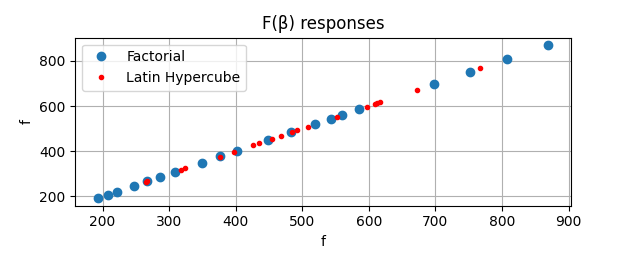
\includegraphics[width=0.6\textwidth]{Figure_31}   
    \caption{Comparison between $\mathbf{F}(\vec{χ})$ 
    responses to samples created via Factorial and LHS DoE scheme}
    \label{fig:Factorial_vs_LHS}
\end{figure}

The two DoE schemes yield similar objective function values, 
as seen in figure \ref{fig:Factorial_vs_LHS}). However, a 
similarity in objective function responses cannot lead to any 
definite conclusions on the quality of the respective models. One 
of many metrics for metamodel quality is the Root Mean Square 
Error (RMSE) (see appendix chapter \ref{appendix:constr_crit}). 
This metric depends on the order of magnitude of the observed 
values and the size of the sample, so it is merely used in the 
comparison of various metamodels when approximating the same PSM 
and trained on the same dataset.  Consequently, a high RMSE is a 
characteristic of a model that has been selectively trained for 
only a narrow set of sample points, therefore lacking in 
robustness. This concept is tested in a KPLS model with fitting  
shown in figure \ref{fig:LHD_FD_training}.

 \begin{figure}[h!]
    \centering
    \begin{subfigure}[b]{0.49\textwidth}
    \centering
    \caption{LHD, NRMSE = 0.003818}
    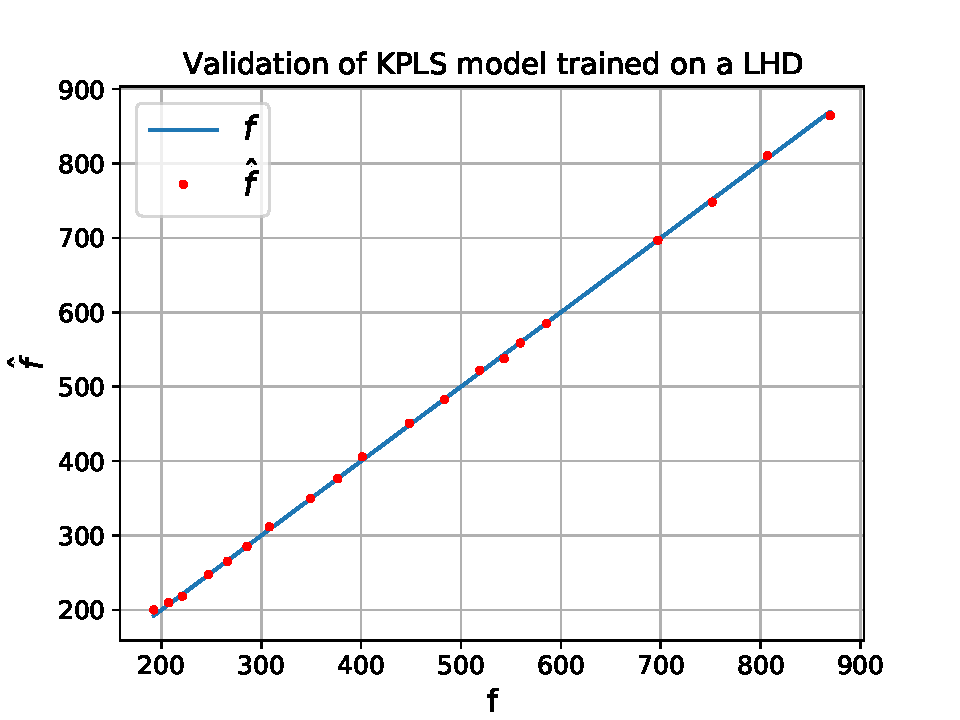
\includegraphics[width=\textwidth, height=0.8\textwidth]
    {Figure_36.pdf} 
    \end{subfigure}  
\hfill
\begin{subfigure}[b]{0.49\textwidth}
    \centering
    \caption{Factorial design, NRMSE = 0.010939}
    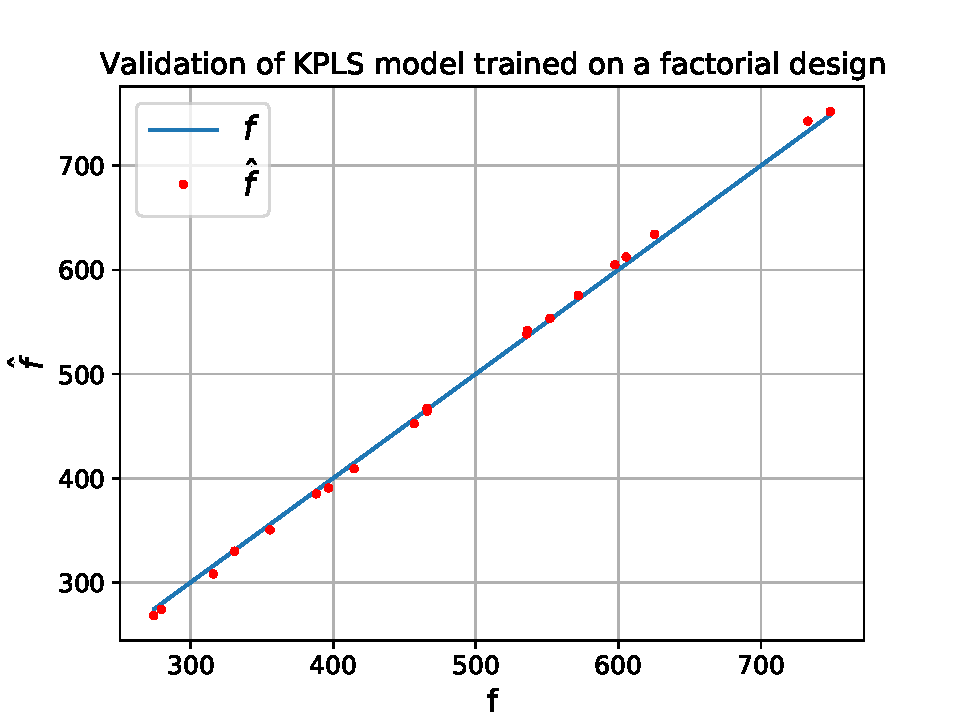
\includegraphics[width=\textwidth, height=0.8\textwidth]
    {Figure_37.pdf} 
    \end{subfigure}
\caption{NRMSE of metamodels trained on a LHD and a factorial 
design}     
\label{fig:LHD_FD_training}  
\end{figure}

\newpage
%------------------------------------------------------


The RMSE is calculated using the following equation:

\begin{equation}\label{RMSE_SOO}
RMSE = \sqrt{ \frac{\sum_{i=1}^{n_{val}} 
\left( \hat{f}_{i} - f_{i} \right)^2 }{n_{val}} }
\end{equation}
\\[0.1cm]
where $n_{val}$ is the number of validation points and   
$\vec{χ_{i}} = \left[ χ_{i,1}, \hdots, χ_{i,n_{β}} \right]
\!\in \!\mathbb{R}^{n_{β}}$ the vector of the $i_{th}$ 
training point. Validation points are selected from the design 
space via the implementation of any DoE technique and are used in 
the evaluation of the model\cite{preprint_SMT}. Every set of 
sample points different than the one used to train the metamodel 
is considered a set of validations point. The values obtained
via the use of the trained surrogate model are denoted by 
$\hat{f}$ and referred to as estimated values. In equation 
\ref{RMSE_SOO} the existence of a single objective is assumed and 
the both $f$ and $\hat{f}$ are scalar quantities. In MOO 
problems, the RMSE is computed w.r.t. to each objective 
iteratively. In order to remove the dependency on the order of 
magnitude Normalised Root Mean Square Error (NRMSE) is 
introduced, which can be calculated from the following formula:
\begin{equation}
NRMSE = \sqrt{ \dfrac{1}{n_{val}}\sum_{i=1}^{n_{val}} \left( 
\frac{ \hat{f}_{i} - f_{i}  }{f_{i}} \right)^2 }
\end{equation}
\\
NRMSE is dimensionless and assumes values in the $\mathbb{R}^{+}$, 
with values closer to zero indicating a well-trained metamodel.
NRMSE is not restricted in a specific dataset but can rather be
generalised to compare models of various orders of magnitude. 

In addition to inferior metamodel quality, factorial designs are 
imposed with severe limitations when sampling high-dimensional 
design spaces. Even in its simplest form a FFD must consist of 
$n_{doe} = 2^{n_{β}}$ possible combinations. In 10 dimensions, 
the number of runs required to fully replicate the design is:
$$ n_{doe} = (2)^{10} = 1024 $$ 

If moreover the case in study is that of a 3D airfoil, then 
each set of design variable values $\vec{β}$ would correspond 
to a different airfoil shape. That results in 1024 
different shapes and therefore to a beyond sustainability 
computational cost. The number of factorial runs needed for the
creation of a factorial design in 10-dimensional space is $n_{doe} 
> 600$, which results experimentally from the implementation Python 
software. On the other hand, LHS scheme is suitable for creating 
high-dimensional designs and offers a better coverage of the design 
space combined with minimal impact on the computational cost, which 
leads to its selection as the main sampling scheme used in this 
thesis. 
   
\newpage
%------------------------------------------------


\section{Communication between EASY and SMT in MAEAs with off-line training}


In the evaluation phase of MAEAs with off-line training the PSM is 
replaced by a surrogate model, which is trained on $n_{t}$ 
training patterns that are collected via the use of various DoE 
techniques. The creation of DoE, the training of the metamodel 
and the prediction of the objective function value are performed 
via the use of SMT. However, in order for SMT to facilitate the 
evolution performed by EASY (see appendix \ref{appendix:EASY}), a 
set of modifications must be applied in order for the two programs 
to be compatible. Responsible for the establishment of a line of 
communication between the two software is a Python script, which is 
manually created and can be decomposed in the following sections:

\begin{enumerate}
\item \textbf{Sampling (Code 1)} \\ 
The design space is defined, i.e. upper and lower bound 
of each design variable, along with the magnitude of the design, 
denoted by $n_{doe}^{'}$, and the DoE technique utilized to 
construct it. The $n_{doe}^{'}$ collected training patterns 
$\mathbf{X}$ are subsequently written in an ASCII text file 
\textit{sample\_points.dat}, prior to the termination of Code 1. 
 
\item \textbf{Evaluation of sample points on the PSM (Code 2)} \\
Code 2 contains the exact PSM. Both the input to the PSM, i.e. 
the observations $\mathbf{X} \! \in \!\mathbb{R}^{n_{doe}^{'} 
\times n_{β}}$ contained in \textit{sample\_points.dat}, and the 
yielded responses $\mathbf{F}(\vec{χ}) \!\in \!\mathbb{R}^{n_{doe}
^{'} \times n}$ are written in a plain ASCII text file 
\textit{model\_values.dat}, along with the constraints $\mathbf{C}
(\vec{χ}) = [\vec{c}_{1}, \vec{c}_{2}, \hdots, \vec{c}
_{n_{t}}]^{T}$, in case the optimization problem is constrained. 
Each component $\vec{c}_{i} = [c_{i,1}, c_{i,2}, \hdots, 
c_{i,n_{c}}]$ corresponds to the constraint vector $\vec{c}
(\vec{χ})$ of the $i_{th}$ sample point $\vec{χ} \in \mathbb{R}
^{n_{β}}$.

\item \textbf{Training of metamodel (Code 3)} \\
Codes 1 through 3 are incorporated in the 
\textit{preprocessor.exe} executable. Code 3 in particular is 
responsible for training the selected surrogate model. In order 
to accomplish that, first $n_{doe}^{'}$ $(\vec{χ}, \vec{f}
(\vec{χ}))$ observed pairs must be imported from 
\textit{model\_values.dat}. At the end of each off-line 
optimization cycle the MDB is updated with $λ_{e}$ elites that 
are contained in the $P_{e}$ set. Consequently, Code 3 is also 
responsible for incorporating $λ_{e}$ $(\vec{β},\vec{f}(\vec{β}))$ 
pairs in the training of the metamodel, after importing them from 
a plain ASCII text file \textit{out.log} that is created by Code 
6. Once the MDB is complete, a new surrogate model is trained at 
the start of each optimization cycle using $n_{t}$ training pairs 
$(\vec{χ},\vec{f}(\vec{χ}))$ (see eq. \ref{off_line_nt}). 

In the case of a constrained optimization, 
the matrix of constraints $\mathbf{C}(\vec{χ})$ is imported 
into Code 3 along with the objective function values 
matrix $\mathbf{F}(\vec{χ})$, and a distinct metamodel is 
trained on each constraint or a single metamodel is trained 
for the entirety of the imposed constraints. Metamodels 
trained on constraints require $n_{t}$ $(\vec{χ},\vec{c}
(\vec{χ}))$ training pairs to be built. 

Once the training is complete, the parameters of each trained 
metamodel are witten in a binary text file using the Python 
module \textit{.pickle()}; in this way, it can be utilized in 
the evaluation of prominent solutions in each generation of the 
evolution. For some metamodels, however, \textit{.pickle()} is not 
applicable, e.g. RBF. In that case, a folder containing the cached 
data that are produced via the training process is used in order 
to store and reuse the saved surrogate model. 

\item \textbf{Evaluation using the trained metamodel 
(Code 4)} \\ 
The current script uses as input the file \textit{task.dat}, which 
EASY creates, and contains a single offspring $\vec{β} \! \in \! 
P_{λ}^g$. A metamodel prediction $\hat{f}(\vec{β})$ is 
subsequently computed for every offspring $\vec{β} \in P_{λ}^g 
\subset \mathbb{R}^{n_{β}}$ by utilizing the stored 
metamodel via the use of \textit{.pickle()} module. Code 4 is 
identical in form to \textit{evaluation.exe}, but the PSM is 
replaced by a surrogate hence it is called 
\textit{prediction.exe}. 

\item \textbf{Selection of objectives and constraints 
(Code 5)} \\
In order to establish the communication between EASY and 
the user, \textit{postprocessor.exe} is manually created. 
This script is responsible for writing the objectives and the 
imposed constraints of the optimization in a \textit{task.cns} 
and a \textit{task.res} file, respectively. Text files 
\textit{task.res} and \textit{task.cns} contain the predictions 
$\hat{\vec{f}}(\vec{β})$ and $\hat{\vec{c}}(\vec{β})$, 
respectively,  of a single individual $\vec{β} \!\in \!P_{λ}^{g}$ 
and are read by EASY.  
 
\item \textbf{Evaluation of elites using the trained 
metamodel (Code 6)} \\
Code 6 performs the evaluation of the elite population 
$P_{e}$ using the exact PSM. The only difference with Code 2 is 
that the inputs $(\vec{β},\hat{\vec{f}}(\vec{β}))$, $(\vec{β},
\hat{\vec{c}}(\vec{β}))$, $\forall \vec{β} \in P_{e}$ are 
imported from \textit{out\_L1.log}, which is created by EASY at 
the end of each optimization cycle, and the corresponding exact 
PSM evaluations $(\vec{β},\vec{f}(\vec{β}))$, $(\vec{β},\vec{c}
(\vec{β}))$ are written in \textit{out.log}. Both these files 
follow ASCII text format.

\end{enumerate}
\newpage
%---------------------------------------------------